% Fig. 1: the closed management loop. Build: pdflatex fig_loop.tex (in paper/figs)
\documentclass[tikz,border=2pt]{standalone}
\usepackage{times}
\usetikzlibrary{arrows.meta,positioning,calc}
\begin{document}
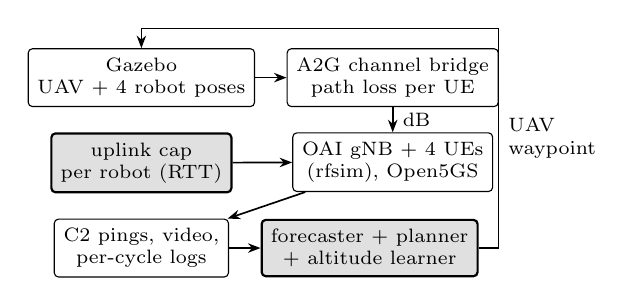
\begin{tikzpicture}[font=\scriptsize, node distance=3.2mm and 4mm,
  box/.style={draw, rounded corners=1.5pt, minimum width=22mm, minimum height=7mm, align=center, fill=white},
  mgmt/.style={box, fill=black!12, thick},
  ar/.style={-{Stealth[length=1.6mm]}, semithick}]
\node[box] (gz) {Gazebo\\UAV + 4 robot poses};
\node[box, right=of gz] (br) {A2G channel bridge\\path loss per UE};
\node[box, below=of br] (ran) {OAI gNB + 4 UEs\\(rfsim), Open5GS};
\node[mgmt, below=of gz] (cap) {uplink cap\\per robot (RTT)};
\node[box, below=of cap] (probe) {C2 pings, video,\\per-cycle logs};
\node[mgmt, right=of probe] (pl) {forecaster + planner\\+ altitude learner};
\draw[ar] (gz) -- (br);
\draw[ar] (br) -- node[right]{dB} (ran);
\draw[ar] (cap) -- (ran);
\draw[ar] (ran) -- (probe);
\draw[ar] (probe) -- (pl);
\draw[ar] (pl.east) -- ++(2.5mm,0) |- node[pos=0.25, right, align=left]{UAV\\waypoint} ($(br.north)+(0,2.5mm)$) -| (gz.north);
\end{tikzpicture}
\end{document}
